\begin{figure*}[htbp]
    \centering
    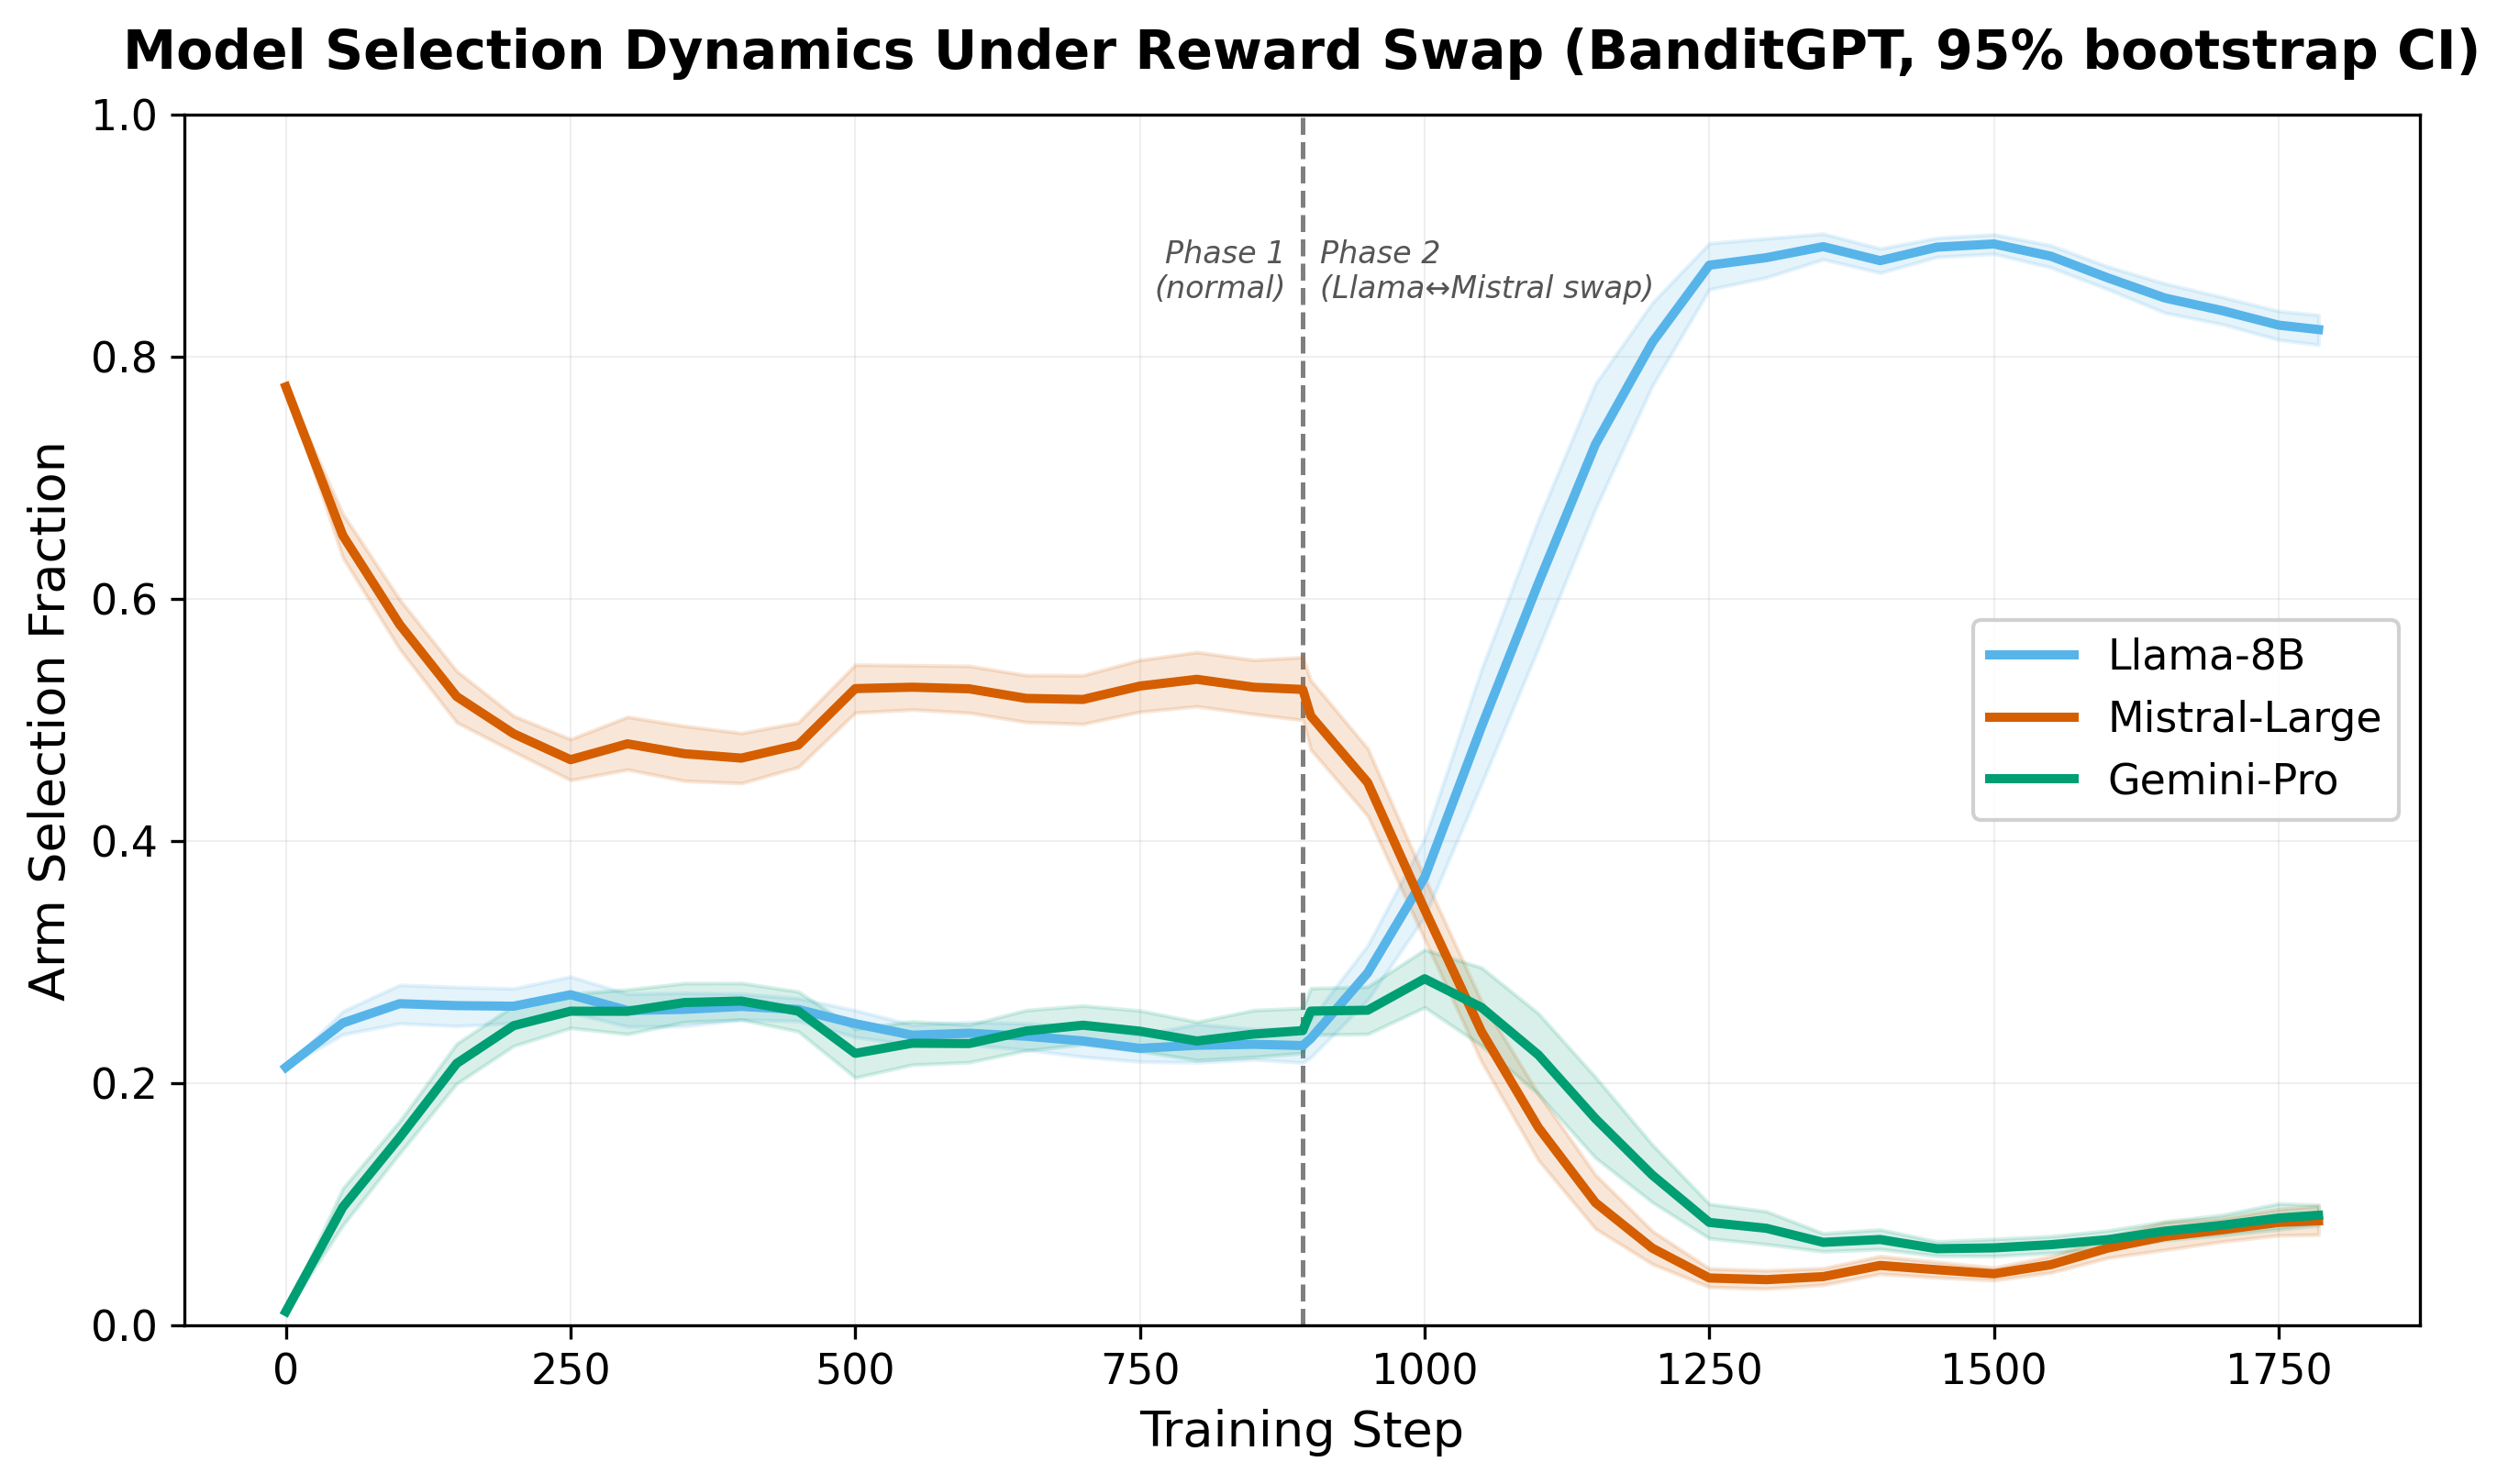
\includegraphics[width=\linewidth]{../experiments/02_nonstationary_k3_drift/results/reward_shift_arm_fractions.pdf}
    \caption{Model selection dynamics under reward swap
    ($K{=}3$; BanditGPT $\gamma{=}0.995$, 40~seeds, $\pm$1\,SD shading).
    %
    Each line shows the fraction of holdout prompts routed to
    each model at every checkpoint, evaluated via frozen
    \texttt{select\_arm()} on the post-swap test set.
    %
    After the reward swap at step~893, BanditGPT shifts
    decisively toward Llama-8B, reaching 81\% Llama allocation
    by step~1{,}785.  The Mistral-Large fraction (orange) shrinks
    rapidly in Phase~2 as the geometric forgetting
    factor~\cite{garivier2011switching} discounts the stale
    Phase~1 evidence that favoured Mistral, while Gemini-Pro
    remains a stable minority allocation.
    }
    \label{fig:arm_fractions}
\end{figure*}
